\section{Approach}
%\rtodo{Claim generality, example with 3 LLMs for illustrative purposes.}

A high level view of our approach is depicted in Figure \ref{fig:ensemble-pipeline}. The first step of the approach includes parsing and static analysis of the COBOL code to understand dependencies among paragraphs, build a call graph, and extract other types of information. 
The output of this step is a set of code chunks, each of which is summarized as a unit in the next steps. Determining the correct granularity of this step is an important aspect of our approach. At one end, chunks at the level of single instructions create verbose descriptions that are not useful. At another extreme, chunks that include whole programs create summaries that hide important details and are not useful. After experimenting with different granularities, we settle for chunks at the paragraph and function level.



Let $C$ denote a COBOL code chunk dedicated to a single functionality. Importantly, the chunking policy is 
\emph{not} under our control: the segmentation into summarisation units 
is predetermined by the Infosys pipeline. Our method therefore treats the 
Infosys chunking as fixed and operates downstream. This constraint reflects 
realistic deployment conditions, where third-party enterprise tooling 
governs preprocessing. 

We assume a set of auxiliary descriptions for called paragraphs or 
programs, $\mathcal{D}=\{(n_i, d_i)\}_{i=1}^{m}$, where $n_i$ is a callee 
name and $d_i$ is a fixed, vetted English description. These include descriptions of called paragraphs/functions. These 
\emph{dependency descriptions} are injected into prompts and 
\emph{not} reconstructed per run, both to reduce variance and to keep the 
evaluation focused on the behaviour of $C$. In addition, the prompt is also augmented with  a list of criteria $L = \{L_1, ..., L_n\}$ specifying the task to the LLM and the outputs (See Appendix for the list used in the evaluation). Specifically, the list $L$ contains the criteria decided by Infosys in their prompt. 
%\rtodo{These are the prompt extensions. Apart from instructions to the LLM about output and behavior, do they include anything else specifically related to the code chunk C?}

We consider three summarisation systems:
\[
M_0=\text{Infosys (OpenAI-based)},\ 
M_1=\text{LLaMA\,3.3-70B},\ 
M_2=\text{Grok-3}.
\]
Given a prompt template aligned with Infosys’ style (to control 
granularity), each model produces a summary:
\[
S_0 \leftarrow M_0(C,\mathcal{D}),\ 
S_1 \leftarrow M_1(C,\mathcal{D}),\ 
S_2 \leftarrow M_2(C,\mathcal{D}).
\]
Model diversity is desirable but the method is agnostic to the specific
choices so long as the models are \emph{competent} summarizers and not
identically trained; the ensemble logic extends to $k>3$ models.

\begin{figure}[t]
  \centering
  \includegraphics[width=0.9\linewidth]{ensemble_pipeline.pdf}
  \caption{Overview of the ensemble-based confidence estimation pipeline. 
           A COBOL code chunk and its dependencies are summarised by three models 
           (Infosys, LLaMA 3.3–70B, Grok–3). Pairwise comparisons with an LLM-as-judge 
           yield structured scores, which are then aggregated into a final confidence estimate.}
  \label{fig:ensemble-pipeline}
\end{figure}


\subsection{Pairwise Evaluation via LLM-as-Judge}
Traditional reference-based metrics (BLEU, ROUGE, BERTScore) correlate
imperfectly with human judgments for code summarisation and are sensitive
to surface form and identifier overlap—a poor fit for reference-free settings.
Prompted LLM judges, by contrast, have shown strong correlation with
human ratings on code tasks \citep{wu2024largelanguagemodelsserve,
robinson2025simpleeffectivebaselinescode}. We therefore instantiate a
dedicated OpenAI model $\mathcal{J}$ as an \emph{evaluator} that compares
pairs of summaries following a list of criteria $L = \{L_1, ..., L_n\}$ specifying the task to the LLM and the outputs (See Appendix for the list used in the evaluation). 

\paragraph{Anchored, pairwise comparisons.}
We conduct two comparisons anchored on the Infosys output:
\[
E_1=\mathcal{J}(S_1, S_0),\qquad E_2=\mathcal{J}(S_2, S_0).
\]
Each evaluation returns a structured JSON record\\
\small
$E_i=(\texttt{agreement}_i,\ \texttt{score}_i,\ 
\texttt{missing\_details}_i,\ \texttt{contradictions}_i,\\ 
\texttt{rationale}_i).
$
\normalsize

The \texttt{agreement} label is one of
\texttt{Agree}/\texttt{Mostly Agree}/\texttt{Disagree}; the
\texttt{score} is a continuous confidence on $[0,10]$ tied to a list of criteria
that emphasises \emph{functional equivalence} (purpose, logic, inputs,
outputs) and discounts mere wording differences. The
\emph{missing-details} and \emph{contradictions} fields enumerate
omissions and logical conflicts, respectively, and the \emph{rationale}
gives a concise justification. These fields serve both downstream
explainability and manual auditability.

\paragraph{Granularity control.}
A common failure mode in pairwise judging is spurious disagreement caused
by \emph{mismatched levels of detail}. To mitigate this, all generators
use prompts that mirror Infosys’ template, and evaluators are instructed
to: (i) ignore stylistic paraphrase; (ii) treat minor omissions as
\texttt{Mostly Agree} if they do not alter semantics; and (iii) reserve
\texttt{Disagree} for contradictions or omissions that change behaviour.
This alignment makes disagreements \emph{diagnostic} rather than an
artefact of verbosity mismatches.

\subsection{Aggregation: Linear Pooling with Conjunctive Penalty}
Let $a_i\in\{\texttt{Agree},\texttt{Mostly Agree},\texttt{Disagree}\}$
and $s_i\in[0,10]$ denote the label and confidence produced by $E_i$.
Define the \emph{support} contributed by each judge as
\[
u_i=\begin{cases}
s_i, & a_i\in\{\texttt{Agree},\texttt{Mostly Agree}\},\\
0,   & a_i=\texttt{Disagree},
\end{cases}
\]
and the \emph{base support} as the linear opinion pool
\[
\bar{u}=\frac{1}{2}(u_1+u_2).
\]
This is the equal-weight linear pool, preserving interpretability (two
10s average to 10) and reflecting the standard practice of combining
expert scores via averaging.

We then apply a \emph{conjunctive penalty} to encode \emph{corroborated}
negative evidence. Let $\mathbf{1}[\cdot]$ be the indicator and define
the \emph{disagreement strength} for a judge as
\[
d_i=\begin{cases}
\frac{5-s_i}{5}\in[0,1], & a_i=\texttt{Disagree},\\
0,                       & \text{otherwise.}
\end{cases}
\]
%\rtodo{This is a weight that influences the strength of the disagreement. Ideally, it will be determined from the evaluation with a ground truth dataset.}
 Intuitively, a \texttt{Disagree} accompanied by $s_i\approx 5$ is weak
($d_i\approx0$), whereas $s_i\approx 0$ is strong ($d_i\approx 1$).
Let $P_{\max}\in[0,5]$ be a hyperparameter. The final score is
\small
\[
\text{Conf} \;=\; \operatorname{clamp}\!\left(
\bar{u}\;-\; \mathbf{1}[a_1=\texttt{Disagree}\wedge a_2=\texttt{Disagree}]
\cdot P_{\max}\cdot \frac{d_1+d_2}{2}\;,\;0,\;10\right)
\]
\normalsize
That is, we \emph{subtract a penalty only if both judges disagree}, and
we scale that penalty by the average strength of their disagreement.
When only one judge disagrees, its support is already zero; we do not
double-penalise, which improves robustness to single-rater noise.
%\rtodo{$P_{max}$ should be determined by evaluation with a ground truth dataset.}


The rule combines two standard ideas: equal-weight \emph{linear opinion
pooling} for supportive evidence and a \emph{$k$-of-$n$ (conjunctive)
decision fusion} for negative evidence. If a false \texttt{Disagree}
occurs with probability $\alpha$ per judge, the chance that both are
false is $\alpha^2$, so penalising only the $2$-of-$2$ case reduces the
expected false penalty from $\alpha$ to $\alpha^2$ under approximate
independence. Empirically, this yields cleaner separation for triage:
cases with two emphatic \texttt{Disagree}s are pushed decisively low,
while “contested” cases (\emph{e.g.}, $10$ vs.\ $5$-\texttt{Disagree})
remain in the middle for human review.

\paragraph{Illustrative outcomes.} With $P_{\max}=3.5$:
\begin{itemize}[nosep]
  \item $(10,\ \texttt{Agree})$ and $(5,\ \texttt{Disagree})$
        $\Rightarrow \bar{u}=5.0$, no penalty $\Rightarrow \text{Conf}=5.0$.
  \item $(3,\ \texttt{Disagree})$ and $(2,\ \texttt{Disagree})$
        $\Rightarrow \bar{u}=0.0$; mean $d=0.5$; penalty $1.75$
        $\Rightarrow \text{Conf}=0.0$ after clamp.
  \item $(5,\ \texttt{Disagree})$ and $(5,\ \texttt{Disagree})$
        $\Rightarrow \bar{u}=0.0$; mean $d=0$; penalty $0$
        $\Rightarrow \text{Conf}=0.0$.
\end{itemize}


\subsection{Token-Level Confidence via Perplexity}
\label{sec:perplexity}

While inter-model agreement provides evidence of semantic consistency, it does not capture
the \emph{generation certainty} of individual summaries. A model may produce a fluent
output that agrees with others yet internally exhibit high uncertainty during generation.
To address this, we incorporate token-level confidence scores derived from the model's
output probability distribution.

\paragraph{Logit probabilities and perplexity.}
Modern LLM APIs support returning log-probabilities for generated tokens when the
\texttt{logprobs} parameter is enabled. For each token $t_i$ in a generated summary
$S = \{t_1, t_2, \dots, t_n\}$, the model provides $\log P(t_i \mid t_{<i}, C)$,
representing the log-probability of token $t_i$ given the preceding context and COBOL
input $C$. We compute the \textbf{perplexity} of a generated summary as
\begin{equation}
\mathrm{PPL}(S) = \exp\!\left(-\frac{1}{n}\sum_{i=1}^{n}\log P(t_i \mid t_{<i}, C)\right).
\label{eq:ppl}
\end{equation}
Perplexity measures how ``surprised'' the model is by its own generation: lower perplexity
indicates higher confidence, while higher perplexity suggests the model struggled to
predict subsequent tokens. For enterprise applications, perplexity provides a
reference-free signal identifying generations where the model exhibited
uncertainty---even if the output appears superficially fluent.

\paragraph{Confidence score normalization.}
Raw perplexity values are model-specific and domain-dependent. We normalize scores to
$[0,10]$ using
\begin{equation}
\mathrm{Conf}_{\mathrm{ppl}}(S) = 10 \times \operatorname{clamp}\!\left(
1 - \frac{\mathrm{PPL}(S) - \mathrm{PPL}_{\min}}{\mathrm{PPL}_{\max} - \mathrm{PPL}_{\min}},\,
0,\, 1\right),
\label{eq:confppl}
\end{equation}
where $\mathrm{PPL}_{\min}$ and $\mathrm{PPL}_{\max}$ are calibrated thresholds from a
held-out validation set of COBOL summaries (Figure~\ref{fig:ppl-norm}). This yields an
interpretable score where $10$ indicates maximum certainty and $0$ indicates the model was
highly uncertain during generation.

\paragraph{Threshold calibration.}
Because perplexity is unbounded on $[1,\infty)$ and its absolute scale varies across
models and domains, raw values are neither directly interpretable nor comparable with the
other $[0,10]$ metrics. The thresholds $\mathrm{PPL}_{\min}$ and $\mathrm{PPL}_{\max}$
anchor the mapping of Equation~\eqref{eq:confppl}: $\mathrm{PPL}_{\min}$ marks the
``confident'' end (mapped to confidence $10$) and $\mathrm{PPL}_{\max}$ the ``uncertain''
end (mapped to confidence $0$), with linear interpolation in between and clamping outside.
Both are estimated from the perplexity distribution over a held-out set of COBOL summaries,
keeping the metric reference-free yet calibrated to the deployment model and corpus.


\begin{figure}[!h]
\centering
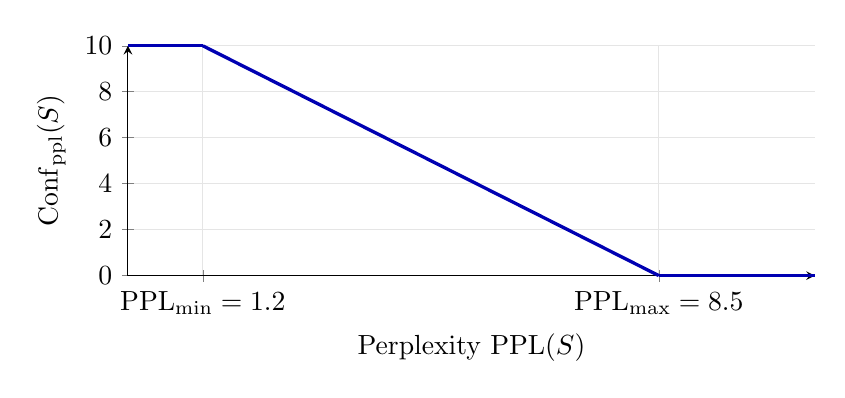
\begin{tikzpicture}
\begin{axis}[
    width=0.85\linewidth, height=4.5cm,
    xlabel={Perplexity $\mathrm{PPL}(S)$},
    ylabel={$\mathrm{Conf}_{\mathrm{ppl}}(S)$},
    xmin=0, xmax=11, ymin=0, ymax=10,
    xtick={1.2,8.5}, xticklabels={$\mathrm{PPL}_{\min}=1.2$,$\mathrm{PPL}_{\max}=8.5$},
    ytick={0,2,4,6,8,10},
    axis lines=left, grid=both, grid style={gray!20},
    every axis plot/.append style={very thick, blue!70!black},
    clip=false,
    legend style={at={(0.95,0.95)}, anchor=north east, draw=none, fill=none},
]
\addplot[domain=0:1.2]   {10};
\addplot[domain=1.2:8.5] {10*(1-(x-1.2)/(8.5-1.2))};
\addplot[domain=8.5:11]  {0};
\end{axis}
\end{tikzpicture}

\caption{Perplexity-to-confidence normalization (Equation~\eqref{eq:confppl}). Summaries with
$\mathrm{PPL} \le \mathrm{PPL}_{\min}$ saturate at maximum score $10$; score decreases
linearly to $0$ at $\mathrm{PPL}_{\max}$ and is clamped beyond. The plot shows: constant
score of $10$ for $\mathrm{PPL} \le 1.2$; linear decrease from $10$ to $0$ over interval
$[1.2, 8.5]$; constant score of $0$ for $\mathrm{PPL} \ge 8.5$.}
\label{fig:ppl-norm}
\end{figure}

\paragraph{Integration with ensemble scores.}
Perplexity complements the inter-model agreement framework:
\begin{itemize}
  \item A summary with high inter-model agreement \textbf{and} low perplexity (high
        $\mathrm{Conf}_{\mathrm{ppl}}$) is strongly validated.
  \item A summary with high inter-model agreement but high perplexity may indicate
        convergence on a challenging interpretation that warrants additional review.
  \item A summary with low inter-model agreement and high perplexity clearly signals
        unreliability.
\end{itemize}
We combine these signals through weighted averaging:
\begin{equation}
\mathrm{Conf}_{\mathrm{base}} = \alpha \cdot \mathrm{Conf} + (1-\alpha) \cdot
\mathrm{Conf}_{\mathrm{ppl}}, \quad \alpha \in [0.6, 0.8],
\label{eq:confbase}
\end{equation}
where $\mathrm{Conf}$ is the aggregated confidence and
$\alpha$ weights ensemble agreement more heavily (as it captures semantic correctness),
while perplexity provides a complementary generation-quality signal.

% ------------------------------------------------------------------
\subsection{Code Coverage Assessment via G-Eval}
\label{sec:coverage}

A critical failure mode unaddressed by pairwise comparison and perplexity is
\textbf{omission}: a model may generate a confident, internally consistent summary that
simply fails to document significant portions of the input code. Reference-based metrics
like BLEU cannot detect omissions without ground-truth coverage annotations. We therefore
introduce a coverage-aware metric adapted from G-Eval \cite{liu2023geval}---a framework
that uses LLMs as evaluators with chain-of-thought reasoning.

\paragraph{G-Eval for summarization coverage.}
Given a COBOL code chunk $C$ and a generated summary $S$, we prompt an LLM evaluator
$\mathcal{E}$ to assess coverage:
\begin{quote}\itshape
``You are an expert code reviewer. Given the following COBOL code and its summary, evaluate
the \textbf{code coverage} of the summary. Code coverage measures whether the summary
accounts for all significant logic: procedure divisions, conditional branches, file I/O
operations, data transformations, and control flow. Identify any code segments omitted by
the summary. Rate coverage on a scale of 1--5:
5: All significant code paths documented;
4: Minor omissions (e.g., edge cases);
3: Moderate omissions;
2: Significant portions undocumented;
1: Summary misses critical logic.
Provide a brief rationale explaining your rating.''
\end{quote}
The evaluator returns a structured response consisting of a coverage score, identified
missing segments, and justification rationale.

\paragraph{Aggregated coverage score.}
To ensure robustness, we query the evaluator $k$ times (temperature $>0$ for diversity)
and aggregate:
\begin{equation}
\mathrm{Cov}(S,C) = \frac{2}{k}\sum_{i=1}^{k}\mathrm{coverage\_score}_i \quad \in [2,10].
\label{eq:cov}
\end{equation}
We use $k=3$ for cost-efficiency while achieving stable estimates (empirically, variance
stabilizes beyond $k=3$). Because each run returns an integer rubric score in
$\{1,\dots,5\}$, with $k=3$ the aggregate takes values in
$\{2.0, 2.67, \dots, 9.33, 10.0\}$; the factor of $2$ rescales the $1$--$5$ scale to
$[2,10]$ for consistency with the other confidence metrics, where higher values indicate
better coverage.

\begin{figure}[!h]
\vspace{0.5cm}
\centering
\begin{tikzpicture}[
    node distance=8mm and 10mm,
    box/.style={draw, rounded corners=2pt, align=center, minimum height=8mm, inner sep=4pt, font=\small},
    io/.style={draw, ellipse, fill=gray!20, align=center, font=\small},
    agg/.style={draw, fill=blue!12, align=center, font=\small},
    arr/.style={-{Latex[length=2mm]}}
]
\node[box] (in) {COBOL chunk $C$ \; + \; summary $S$};
\node[box, below=of in] (prompt) {G-Eval coverage prompt\\(1--5 rubric + criteria)};
\node[box, below=12mm of prompt] (e1) {Eval run $2$};
\node[box, left=of e1] (e0) {Eval run $1$};
\node[box, right=of e1] (e2) {Eval run $k$};
\node[agg, below=12mm of e1] (agg) {$\displaystyle \mathrm{Cov}(S,C)=\tfrac{2}{k}\sum_{i=1}^{k}\mathrm{cov}_i \in [2,10]$};
\node[io, below=of agg] (out) {$\mathrm{Conf}_{\text{final}}=\mathrm{Conf}_{\text{base}} \times \tfrac{\mathrm{Cov}(S,C)}{10}$};
\draw[arr] (in)--(prompt);
\draw[arr] (prompt)--(e0);
\draw[arr] (prompt)--(e1);
\draw[arr] (prompt)--(e2);
\draw[arr] (e0)--(agg);
\draw[arr] (e1)--(agg);
\draw[arr] (e2)--(agg);
\draw[arr] (agg)--(out);
\end{tikzpicture}
\vspace{-0.3cm}
\caption{Coverage assessment via G-Eval. The (chunk, summary) pair is scored $k$ times
($\tau > 0$) on a 1--5 rubric; scores are averaged and rescaled to $[2,10]$
(Equation~\eqref{eq:cov}), then applied as multiplicative penalty to base confidence
(Equation~\eqref{eq:conffinal}).}
\label{fig:geval}
\end{figure}

\paragraph{Detection of systematic omissions.}
Beyond numerical scores, G-Eval's rationale field enables qualitative analysis. If
multiple evaluations identify the same missing segments (e.g., ``file error handling not
mentioned''), this provides actionable feedback for human reviewers or model fine-tuning.

\paragraph{Why G-Eval over heuristics?}
Naive coverage metrics might count lines of code mentioned or perform keyword matching
(e.g., checking if all COBOL verbs appear in the summary). However, such heuristics fail
to capture semantic coverage: a summary might mention ``file operations'' without
explaining what those operations do. G-Eval's LLM-based evaluation reasons about semantic
completeness rather than surface-level lexical overlap, aligning with our goal of
reference-free semantic assessment.

\paragraph{Integration with confidence framework.}
The coverage score penalizes the final confidence estimate when summaries exhibit
omissions:
\begin{equation}
\mathrm{Conf}_{\mathrm{final}} = \mathrm{Conf}_{\mathrm{base}} \times
\frac{\mathrm{Cov}(S,C)}{10}.
\label{eq:conffinal}
\end{equation}
This multiplicative penalty ensures that even high-agreement, low-perplexity summaries
receive reduced confidence if they fail to cover critical code paths. For example, a
summary scoring $\mathrm{Conf}_{\mathrm{base}} = 8.5$ but $\mathrm{Cov} = 4$ yields
$\mathrm{Conf}_{\mathrm{final}} = 3.4$, correctly flagging incomplete documentation.


\subsection{System Design and Prompts}
\paragraph{Generation stage.}
Each model receives a prompt that: (i) includes the code chunk $C$ and
the fixed set $\mathcal{D}$; (ii) requests a concise English summary
focused on purpose, control-flow conditions, inputs/outputs, and state
effects; and (iii) mirrors the Infosys formatting conventions to enforce
granularity compatibility.

\paragraph{Evaluation stage.}
The evaluator prompt instructs $\mathcal{J}$ to compare two descriptions
strictly on semantics, to classify agreement levels, to assign a
0–10 confidence, and to output \emph{only} a JSON object with fields
\texttt{agreement}, \texttt{confidence\_score},
\texttt{missing\_details}, \texttt{contradictions}, \texttt{rationale}.
This schema yields machine-parsable signals and high-quality natural-
language rationales for explainability.

\paragraph{Engineering notes.}
We set deterministic decoding for evaluators (temperature~$=0$) to
stabilise judgments; generators may use mild stochasticity to improve
diversity if $k>3$. We implement strict JSON validation with
auto-repair on recoverable formatting errors. Since $\mathcal{D}$ is
static, we cache its tokenisation to control costs and latency.


\subsection{Complexity, Cost, and Extensibility}
For each code chunk, the minimal configuration incurs: two non-Infosys
generations ($M_1,M_2$) and two evaluations ($\mathcal{J}$), plus the
Infosys summary if not already available. The approach scales to $k>3$
by (i) averaging supports from $k-1$ comparators against the anchor; and
(ii) generalising the penalty to a $k$-of-$(k-1)$ rule (\emph{e.g.},
penalise if at least two judges \texttt{Disagree}), tuned to desired
conservatism. Full pairwise all-to-all comparisons are possible but
increase cost quadratically.

\subsection{Threats to Validity and Mitigations}
\paragraph{Correlated model errors.}
If models share blind spots (training data, instructions), agreement may
over-estimate correctness. \emph{Mitigation:} diversify families (open-
weights vs.\ proprietary), decode settings, and prompting styles.

\paragraph{Anchor bias.}
Anchoring on $S_0$ risks propagating its idiosyncrasies.
\emph{Mitigation:} periodically rotate anchors, or include a lightweight
cross-check where $\mathcal{J}$ also compares $(S_1,S_2)$ to detect
transitivity violations.
%(TODO: review this, it's relevant, but might be out of scope since the purpose is specifically to evaluate infosys summary)

\paragraph{Granularity drift.}
Even with matched templates, certain COBOL patterns (nested PERFORM,
COPY expansions) induce verbosity differences that look
like omissions. \emph{Mitigation:} expand the framework with
pattern-specific guidance and augment prompts with static-analysis facts
when available.

%\paragraph{Evaluator bias.}
